\documentclass[tikz,border=5mm]{standalone}
\usepackage[T1]{fontenc}
\usepackage{lmodern}
\usepackage{amsmath,amssymb}
\usepackage{xcolor}
\usepackage{tikz}
\usetikzlibrary{arrows.meta,positioning,calc,fit,backgrounds,decorations.pathreplacing,shapes.geometric}
\tikzset{
  doc/.style = {rectangle, draw, rounded corners=2pt, minimum width=1.1cm, minimum height=0.62cm, inner sep=2pt, fill=white},
  sum/.style = {rectangle, draw, rounded corners=3pt, inner sep=4pt, fill=green!6},
  plus/.style = {circle, draw, minimum size=0.4cm, inner sep=0pt, fill=white},
  chip/.style = {rectangle, rounded corners=3pt, minimum width=1.95cm, minimum height=0.72cm, inner sep=3pt},
  panel/.style = {rounded corners=4pt, line width=0.9pt},
}
\definecolor{regA}{HTML}{4C78A8}
\definecolor{regB}{HTML}{F58518}
\definecolor{regC}{HTML}{54A24B}
\definecolor{regD}{HTML}{E45756}
\begin{document}
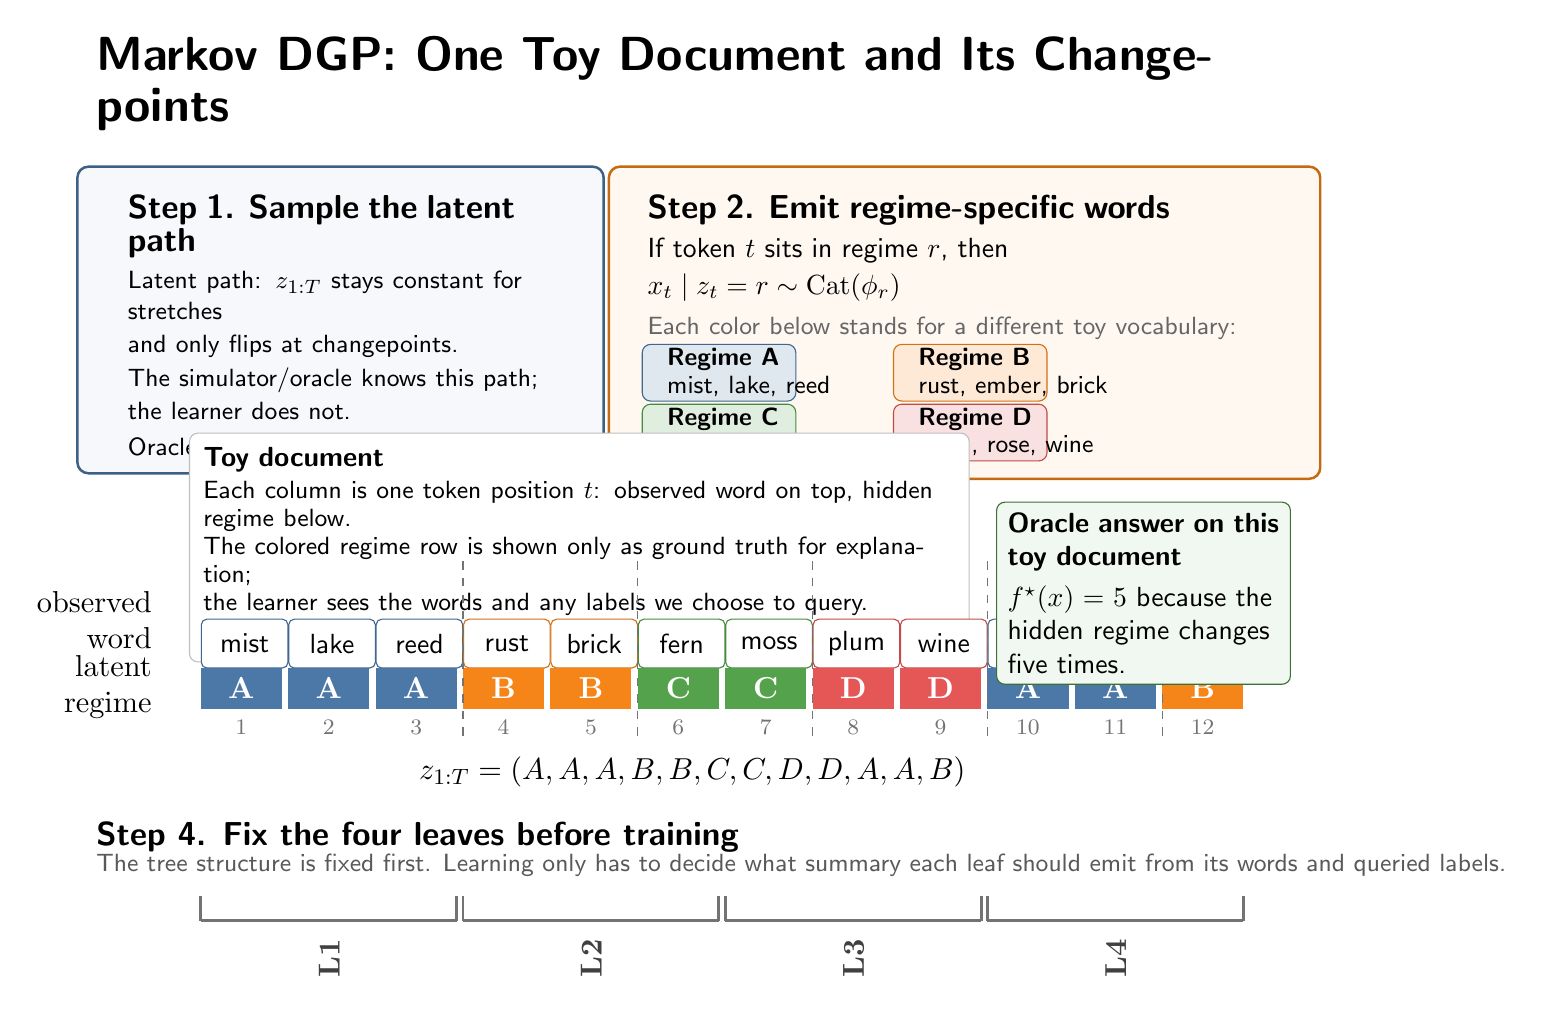
\begin{tikzpicture}[x=1cm,y=1cm,font=\sffamily]
  \node[anchor=west, align=left, text width=15.5cm, font=\sffamily\bfseries\fontsize{16.5}{18.5}\selectfont] at (0, 8.45)
    {Markov DGP: One Toy Document and Its Changepoints};

  \node[anchor=north west, align=left, text width=5.7cm, font=\sffamily] at (0.40, 7.16)
     {{\bfseries\fontsize{11.6}{13.6}\selectfont Step 1. Sample the latent path}\\[0.8mm]
     {\fontsize{9.4}{11.1}\selectfont Latent path: $z_{1:T}$ stays constant for stretches\\and only flips at changepoints.}\\[0.45mm]
     {\fontsize{9.2}{10.9}\selectfont The simulator/oracle knows this path;\\the learner does not.}\\[0.45mm]
     {\fontsize{9.4}{11.1}\selectfont Oracle target: count the regime flips.}};
  \begin{scope}[on background layer]
    \node[panel, draw=regA!80!black, fill=regA!5, fit={(0.0,3.62) (6.45,7.28)}] {};
  \end{scope}

  \node[anchor=north west, align=left, text width=7.95cm, font=\sffamily] at (7.00, 7.16)
    {{\bfseries\fontsize{11.6}{13.6}\selectfont Step 2. Emit regime-specific words}\\[0.8mm]
     {\fontsize{9.8}{11.8}\selectfont If token $t$ sits in regime $r$, then}\\[0.5mm]
     {\fontsize{10.4}{12.4}\selectfont $x_t \mid z_t=r \sim \mathrm{Cat}(\phi_r)$}\\[0.8mm]
     {\fontsize{8.9}{10.9}\selectfont\color{black!60} Each color below stands for a different toy vocabulary:}};
  \node[chip, draw=regA!85!black, fill=regA!18, anchor=west] at (7.05, 4.78) {};
  \node[chip, draw=regB!85!black, fill=regB!18, anchor=west] at (10.24, 4.78) {};
  \node[chip, draw=regC!85!black, fill=regC!18, anchor=west] at (7.05, 4.02) {};
  \node[chip, draw=regD!85!black, fill=regD!18, anchor=west] at (10.24, 4.02) {};
  \node[anchor=west, font=\sffamily\bfseries\fontsize{9.3}{10.7}\selectfont] at (7.25, 4.95) {Regime A};
  \node[anchor=west, font=\sffamily\fontsize{8.6}{10.0}\selectfont] at (7.25, 4.60) {mist, lake, reed};
  \node[anchor=west, font=\sffamily\bfseries\fontsize{9.3}{10.7}\selectfont] at (10.44, 4.95) {Regime B};
  \node[anchor=west, font=\sffamily\fontsize{8.6}{10.0}\selectfont] at (10.44, 4.60) {rust, ember, brick};
  \node[anchor=west, font=\sffamily\bfseries\fontsize{9.3}{10.7}\selectfont] at (7.25, 4.19) {Regime C};
  \node[anchor=west, font=\sffamily\fontsize{8.6}{10.0}\selectfont] at (7.25, 3.84) {fern, moss, leaf};
  \node[anchor=west, font=\sffamily\bfseries\fontsize{9.3}{10.7}\selectfont] at (10.44, 4.19) {Regime D};
  \node[anchor=west, font=\sffamily\fontsize{8.6}{10.0}\selectfont] at (10.44, 3.84) {plum, rose, wine};
  \begin{scope}[on background layer]
    \node[panel, draw=regB!80!black, fill=regB!6, fit={(6.75,3.55) (15.55,7.28)}] {};
  \end{scope}

  \node[sum, draw=black!25, fill=white, anchor=west, text width=9.55cm, inner sep=5pt] at (1.30, 2.56)
    {{\bfseries\fontsize{10.2}{11.8}\selectfont Toy document}\\[0.6mm]
    {\fontsize{8.55}{10.05}\selectfont Each column is one token position $t$: observed word on top, hidden regime below.\\
    The colored regime row is shown only as ground truth for explanation;\\
    the learner sees the words and any labels we choose to query.\\
    Dashed lines mark the five true changepoints.}};
  \node[anchor=east, align=right, font=\fontsize{11}{13}\selectfont] at (0.95, 1.64) {observed\\word};
  \node[anchor=east, align=right, font=\fontsize{11}{13}\selectfont] at (0.95, 0.79) {latent\\regime};

  \foreach \w/\r/\c/\x in {
    mist/A/regA/1.45,
    lake/A/regA/2.56,
    reed/A/regA/3.67,
    rust/B/regB/4.78,
    brick/B/regB/5.89,
    fern/C/regC/7.00,
    moss/C/regC/8.11,
    plum/D/regD/9.22,
    wine/D/regD/10.33,
    lake/A/regA/11.44,
    mist/A/regA/12.55,
    ember/B/regB/13.66
  }{
    \node[doc, draw=\c!85!black, anchor=west] at (\x, 1.34) {\w};
    \fill[\c] (\x, 0.51) rectangle ++(1.03, 0.52);
    \node[font=\bfseries\fontsize{11}{12}\selectfont, text=white] at (\x+0.515, 0.77) {\r};
  }
  \foreach \n/\x in {1/1.965,2/3.075,3/4.185,4/5.295,5/6.405,6/7.515,7/8.625,8/9.735,9/10.845,10/11.955,11/13.065,12/14.175}{
    \node[font=\fontsize{8.5}{9.5}\selectfont, text=black!55] at (\x, 0.27) {\n};
  }
  \foreach \x in {4.78,7.00,9.22,11.44,13.66}{
    \draw[dashed, black!55] (\x, 0.17) -- (\x, 2.40);
  }
  \node[sum, draw=regC!70!black, fill=regC!8, anchor=west, text width=3.45cm] at (11.55, 1.98)
    {\textbf{Oracle answer on this toy document}\\[1mm]$f^\star(x)=5$ because the hidden regime changes five times.};
  \node[anchor=west, font=\fontsize{11}{13}\selectfont] at (4.1, -0.29)
    {$z_{1:T}=(A,A,A,B,B,C,C,D,D,A,A,B)$};

  \node[anchor=west, font=\sffamily\bfseries\fontsize{13}{15}\selectfont] at (0, -1.12)
    {Step 4. Fix the four leaves before training};
  \node[anchor=west, text=black!65, font=\sffamily\fontsize{9.2}{11.2}\selectfont] at (0, -1.48)
    {The tree structure is fixed first. Learning only has to decide what summary each leaf should emit from its words and queried labels.};

  \foreach \left/\right/\mid/\lab in {
    1.45/4.70/3.08/L1,
    4.78/8.03/6.41/L2,
    8.11/11.36/9.74/L3,
    11.44/14.69/13.07/L4
  }{
    \draw[black!55, line width=1.05pt] (\left,-1.86) -- (\left,-2.18);
    \draw[black!55, line width=1.05pt] (\left,-2.18) -- (\right,-2.18);
    \draw[black!55, line width=1.05pt] (\right,-1.86) -- (\right,-2.18);
    \node[font=\bfseries\fontsize{10.5}{11.5}\selectfont, text=black!75, rotate=90] at (\mid, -2.66) {\lab};
  }
\end{tikzpicture}

\end{document}
